\chapter{Introducción}
En el contexto tecnológico actual, en donde el Big Data es un recurso cada vez más
utilizado, el rol del analista de datos (data scientist) se está convirtiendo en una profesión
emergente y de elevada demanda. Un analista de datos es aquel que reúne, analiza e interpreta
los datos obtenidos con el objetivo de sacar ciertas conclusiones de ellos y así tomar diferentes
decisiones, con las que aumentar la productividad. El analista de datos combina diferentes
habilidades, especialmente las técnicas de la minería de datos y del aprendizaje automático (DM\&M).

Según Mitchell \cite{mitchell}, una definición de aprendizaje automático sería la siguiente: Un programa de
ordenador aprende a partir de una experiencia E a realizar una tarea T (de acuerdo con una medida
de rendimiento P), si su rendimiento al realizar T, medido con P, mejora gracias a la experiencia E.

Una de las tareas más importantes que se deben llevar a cabo es la validación de resultados
obtenidos por los algoritmos de aprendizaje. El método estándar más aceptado en la actualidad
es el de la aplicación de test estadísticos sobre los experimentos, que, entre otras utilidades,
apoyan la toma de decisiones (por ejemplo la elección del algoritmo más adecuado).

Este proyecto se centra en crear y desarrollar una interfaz web para asistir al analista de
datos en el proceso de validación de resultados. En este proyecto se desarrollará una plataforma web
y se extenderá una librería de tests estadísticos con el objetivo de que el analista de datos
pueda introducir en la web los datos obtenidos y seleccionar el test estadístico que desea
utilizar para que, de forma automática, el sistema devuelva los resultados obtenidos después de
la aplicación del test. Así, el sistema permitirá de un modo fácil y centralizado la utilización de
tests estadísticos.

La herramienta se incorporará en la lista de aplicaciones disponibles a través de la web del
CiTIUS para su uso. El impacto y difusión del resultado del proyecto va a ser amplio, ya que en la
actualidad no existe ninguna herramienta que centralice la aplicación de los test estadísticos de mayor
utilidad y que resulte fácil de usar.

\section{Objetivos del proyecto}
El proyecto se centra en crear y desarrollar una plataforma web para asistir al analista de datos
en el proceso de validación de resultados obtenidos de diferentes algoritmos de aprendizaje.
Para ello, habrá que desarrollar tres componentes diferenciados:
\begin{enumerate}
\item Completar y extender una librería de test estadísticos, actualmente implementada en el
lenguaje Python.
\item Crear los servicios web en Python, basados en REST, que hagan disponible el acceso a los
tests estadísticos vía web.
\item Desarrollar una interfaz web (HTML + JavaScript) para facilitar el uso de los tests sobre los
datos introducidos por el analista de datos.
\end{enumerate}

\section{Contraste de hipótesis}
El contraste de hipótesis, o lo que se conoce como tests estadísticos se engloba dentro de la rama de la
estadística: \textit{Inferencia Estadística}, que es una parte de la estadística que estudia cómo sacar
conclusiones generales (sujetas a un determinado grado de fiabilidad o significancia) para toda la población
a partir del estudio de una muestra. En nuestro caso, se tratará de sacar conclusiones de los resultados
obtenidos por diferentes algoritmos (muestra) para determinar por ejemplo si los algoritmos tienen un
rendimiento similar y por lo tanto se pueden considerar iguales (población).

El contraste de hipótesis es uno de los problemas más comunes dentro de la inferencia estadística. En él se
contrasta una hipótesis estadística. Por ejemplo:\\\\
\textit{Un ingeniero de software afirma que la media de los resultados obtenidos por un algoritmo
de aprendizaje automático es 10. ¿Se podría desmentir la afirmación del ingeniero?}\\\\
El planteamiento del contraste sería el siguiente:
\begin{center}
$ \mu = 10 $

$ \mu \neq 10 $
\end{center}

Para tomar una decisión (desmentir o no la afirmación), habría que basarse en los datos de una muestra, y
ver si en efecto la media de los resultados es 10. Se podría establecer una regla de decisión sobre la cual
se basaría nuestra decisión final. Por ejemplo: si la media obtenida está próxima a la afirmada por el
ingeniero (10), entonces se podría afirmar dice la verdad. Si por el contrario la muestra nos proporciona
una media muy distinta a 10, entonces se diría que el ingeniero miente sobre el algoritmo en cuestión. Esto
supone un problema y es el hecho de cuándo considerar que la media es lo suficientemente distinta como para
determinar que la afirmación del ingeniero es errónea. Por ejemplo si la media de la muestra es 8.5, ¿se
podría desmentir la afirmación inicial? El contraste de hipótesis nos proporciona una forma de establecer
este criterio y poder rechazar o aceptar la afirmación inicial.

\subsection{Hipótesis nula y alternativa}
En todo contraste de hipótesis siempre siempre se dan dos posibilidades o hipótesis, las cuales se representan
con los siguientes símbolos:
\begin{center}
$H_0:$ Hipótesis nula

$H_1:$ Hipótesis alternativa
\end{center}
A modo de ejemplo, supongamos que unos programadores están trabajando en la optimización de un algoritmo
de aprendizaje. El objetivo es mejorar el algoritmo de forma que los resultados que proporcione sean menores
de 100. Se toma una muestra de los resultados obtenidos por el nuevo algoritmo optimizado y se observa que la
media de la muestra es de 92. Si no hubiera incertidumbre en la media muestral, entonces se podría concluir
que la modificación reduciría los resultados a 92. Sin embargo, siempre existe incertidumbre en la media
muestral. La media poblacional en realidad será poco mayor o menor a 92.

Los programadores están preocupados de que el nuevo algoritmo en realidad no mejore al anterior, es decir, que
la media poblacional pudiera ser mayor o igual a 100. Quieren saber si esta preocupación está justificada. Se ha
observado una muestra con media de 92 y existen dos posibles interpretaciones o, como se ha mencionado más arriba
dos tipos de hipótesis que serán contrastadas más adelante mediante un determinado test estadístico:
\begin{enumerate}
\item La media poblacional es mayor o igual a 100 (la media muestral es, por tanto, menor debido sólo a la
variación aleatoria de la media poblacional). El nuevo algoritmo no mejorará al anterior.
\item La media poblacional es menor que 100, y la media muestral lo refleja. El nuevo algoritmo sí mejorará
al anterior.
\end{enumerate}
La primera interpretación sería la hipótesis nula o $H_0$, que es la hipótesis que se supone cierta de partida, es
decir, es la hipótesis que establece que lo que indica la muestra es solamente debido a la variación aleatoria entre
la muestra y la población. La segunda interpretación o $H_1$, es la hipótesis alternativa y es la que reemplazará a
la hipótesis nula si ésta es rechazada. $H_1$ establece que lo que indica la muestra es verdadero, ya que representa
a toda la población.

En este caso, los programadores están preocupados de que la hipótesis nula sea cierta. Un test estadístico o prueba
de hipótesis hallará, entre otras cosas  una medida cuantitativa de la factibilidad de la hipótesis nula (denominado estadístico de contraste) y se podrá decir a los programadores (después de que el test tome la decisión) si su
preocupación está o no justificada. Por tanto, a modo de resumen este ejemplo nos proporciona dos hipótesis:
$$H_0: \mu \geq 100 \mbox{ vs. } H_1: \mu < 100$$

La realización de un contraste de hipótesis no consiste en decidir cuál de las dos hipótesis ($H_0$, $H_1$) es más
creíble, sino en decidir si la muestra proporciona o no suficiente evidencia para descartar $H_0$. Para realizar la
prueba de hipótesis o test estadístico se pone la hipótesis nula en juicio, es decir se empieza suponiendo que $H_0$
es verdadera. Se podría poner como analogía el supuesto de \textit{``En un juicio, el acusado siempre es inocente
hasta que se demuestre lo contrario."} Es decir:
\begin{center}
$H_0:$ El acusado es inocente

$H_1:$ El acusado es culpable
\end{center}
y, mientras no se tenga suficiente evidencia para aceptar $H_1$, hay que creer que lo que dice $H_0$ es cierto. La
muestra aleatoria proporcionará la evidencia. Si el juicio (test o prueba de hipótesis) determina que el acusado
es inocente, sólo se puede decir que no se tiene suficiente evidencia para asegurar que el acusado es culpable,
mientras que si aceptamos la hipótesis alternativa, se estará bastante seguro de que el acusado sí es culpable.

\subsection{Decisiones y tipos de error}
Cuando se lleva a cabo un contraste de hipótesis sólo se pueden tomar dos decisiones. Los datos de la muestra,
evidenciarán qué decisión se debe tomar:
\begin{enumerate}
\item Aceptar la hipótesis nula ($H_0$) (Rechazar la hipótesis alternativa $H_1$)
\item Rechazar $H_0$ (Aceptar la hipótesis alternativa)
\end{enumerate}
\begin{figure}[h]
\centering
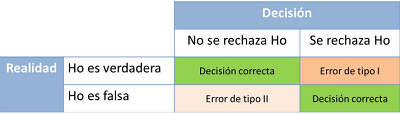
\includegraphics[height=2.5cm]{figuras/figura1.png}
\caption{Decisiones y tipos de error.}
\label{fig:decision}
\end{figure}
La muestra, en el caso de este proyecto, vendrá dada por los resultados obtenidos por los algoritmos. Sin embargo,
cuando se toma la decisión se pueden cometer dos tipos de error. La figura \ref{fig:decision}, nos muestra las
decisiones y los dos tipos de errores que se pueden cometer.

Se puede tomar una decisión correcta o errónea. La probabilidad de \textit{``Error tipo I"} se denota por $\alpha$
y se denomina nivel de significación:
\begin{center}
$P(\mbox{Error tipo I}) = P(\mbox{Rechazar } H_0|H_0 \mbox{ es cierta}) =\alpha.$
\end{center}
La probabilidad de \textit{``Error tipo II"} se denota por $\beta$:
\begin{center}
$P(\mbox{Error tipo II}) = P(\mbox{Aceptar } H_0|H_0 \mbox{ es falsa}) =\beta.$
\end{center}
Por otra parte, la \textit{``Potencia"} es la probabilidad de detectar que una hipótesis es falsa. Los tests
estadísticos o pruebas de hipótesis implementados en el presente proyecto serán mejores o peores dependiendo
de su potencia:
\begin{center}
$P(\mbox{Potencia}) = P(\mbox{Rechazar } H_0|H_0 \mbox{ es falsa}) =1-\beta.$
\end{center}

El \textit{``Error tipo I"}, es lo más peligroso que puede ocurrir, mientras que el \textit{``Error tipo II"}
no es tan importante. Volviendo al ejemplo de la analogía del juicio, es mucho peor condenar a un inocente que
absolver a un culpable. Obviamente, lo ideal sería que tanto $\alpha$ como $\beta$ fuesen nulos y que no se
cometiese ningún error, o que ambos valores fuesen muy pequeños. Como no se pueden disminuir ambos errores a la
vez, se controla el \textit{``Error tipo I"}, que es el más importante.

%\subsection{Etapas en la resolución de un contraste de hipótesis}
%\subsection{Tests paramétricos y no paramétricos}
%\subsection{Concepto de p-valor}
%\section{Organización del documento}